\documentclass{beamer}
% Replace the \documentclass declaration above
% with the following two lines to typeset your 
% lecture notes as a handout:
%\documentclass{article}
\usepackage{CJKutf8}
\usepackage[T1]{fontenc}
%\usepackage[utf8x]{inputenc}
\usepackage{graphicx}
\usepackage{subfigure}
\usepackage{mathtools}
\usepackage{ulem}
\usepackage{url}
\usepackage{pifont}

\everymath{\displaystyle}

% There are many different themes available for Beamer. A comprehensive
% list with examples is given here:
% http://deic.uab.es/~iblanes/beamer_gallery/index_by_theme.html
% You can uncomment the themes below if you would like to use a different
% one:
%\usetheme{AnnArbor}
%\usetheme{Antibes}
%\usetheme{Bergen}
%\usetheme{Berkeley}
%\usetheme{Berlin}
%\usetheme{Boadilla}
%\usetheme{boxes}
%\usetheme{CambridgeUS}
%\usetheme{Copenhagen}
%\usetheme{Darmstadt}
%\usetheme{default}
%\usetheme{Frankfurt}
%\usetheme{Goettingen}
%\usetheme{Hannover}
%\usetheme{Ilmenau}
%\usetheme{JuanLesPins}
%\usetheme{Luebeck}
%\usetheme{Madrid}
%\usetheme{Malmoe}
%\usetheme{Marburg}
%\usetheme{Montpellier}
%\usetheme{PaloAlto}
%\usetheme{Pittsburgh}
%\usetheme{Rochester}
%\usetheme{Singapore}
%\usetheme{Szeged}
\usetheme{Warsaw}

\begin{document}
\begin{CJK}{UTF8}{gbsn}

\title{度假搜索业务目标与原则简介}

% A subtitle is optional and this may be deleted
\subtitle{Q3,Q4工作重点}

\author{李庚\inst{1}}
% - Give the names in the same order as the appear in the paper.
% - Use the \inst{?} command only if the authors have different
%   affiliation.

\institute[Qunar.com] % (optional, but mostly needed)
{
  \inst{1}
  旅游度假事业部-搜索及频道 \\
  Qunar.com
}
% - Use the \inst command only if there are several affiliations.
% - Keep it simple, no one is interested in your street address.

\date{\today}

\AtBeginSubsection[]
{
  \begin{frame}<beamer>{纲要}
    \tableofcontents[currentsection,currentsubsection]
  \end{frame}
}

\begin{frame}
  \titlepage
\end{frame}

\begin{frame}{纲要}
  \tableofcontents
  % You might wish to add the option [pausesections]
\end{frame}

\section{2015上半年总结}

\begin{frame}{2015上半年工作总结}
  \begin{columns}
    \column{0.4\textwidth}
    \begin{center}
      \uncover<2> {
\includegraphics[scale=0.5]{./images/product-scale}}
      \uncover<4> {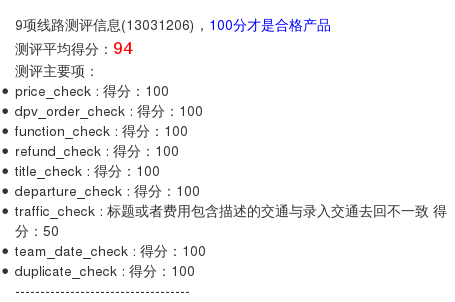
\includegraphics[scale=0.3]{./images/route-quality}}
    \end{center}
    \column{0.6\textwidth}
    \begin{enumerate}[1]
      \item<2> 支持的独立产品规模:60万 \ding{213} 100万+
      \item<3> SEO初见成效:百度日均带来18k独立用户访问
      \item<4> 数据抽取质量评测形成规范流程
    \end{enumerate}
  \end{columns}
\end{frame}

\begin{frame}{2015上半年工作总结}
  \begin{columns}
    \column{0.4\textwidth}
    \begin{center}
      \begin{minipage}[b]{1\textwidth}
        \uncover<2> {
          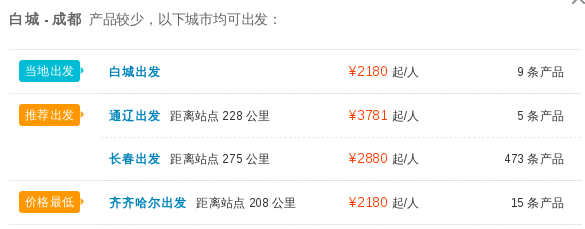
\includegraphics[scale=0.2]{./images/dep-recommend}\\
          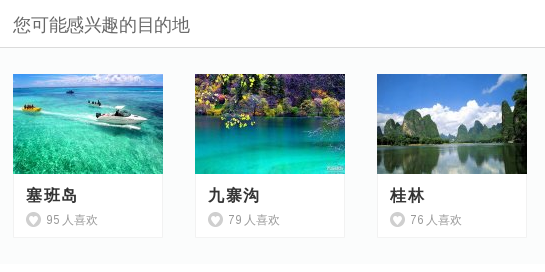
\includegraphics[scale=0.2]{./images/dest-recommend}
        }
        \uncover<4> {
          
\includegraphics[scale=0.4]{./images/a}\\
          
\includegraphics[scale=0.4]{./images/b}
        }
      \end{minipage}
    \end{center}
    \column{0.6\textwidth}
    \begin{enumerate}\setcounter{enumi}{3}
      \item<2> 搜索相关推荐算法使用范围推广:出发地、目的地推荐、详情页相关产品推荐
      \item<3> Qsearch基础依赖升级:Lucene 3 \ding{213} Lucene 4
      \item<4> 小流量测试环境投入使用
    \end{enumerate}
  \end{columns}
\end{frame}


\section{度假事业部业务概述}

\begin{frame}{为什么要做上面的工作?}
  \uncover<2-> {
    事业部要解决的问题:整合供应商提供的产品,满足用户的出行需求。\\
    两个重要的量化指标:
  }
  \begin{itemize}
    \item<3-> { GMV: Gross Merchandise Value,总交易额 }
    \item<4-> { 毛利:$GMV - \text{成本} $ }
  \end{itemize}
\end{frame}

\begin{frame}{GMV量化分析方法}

  \begin{itemize}
  \item<2-> { UV: 独立用户访问量 }
  \item<3-> { \color<9>{blue}{ A: 服务可用率 } }
  \item<4-> { \color<9>{blue}{ R: UV至订单转化率 } }
  \item<5-> { M: 平均用户交易额 }
  \item<7-> { S: 访问来源 }
  \end{itemize}
  
  \uncover<6-7>{
    $$  UV \times A \times R \times M $$
  }
  \uncover<8->{
    $$  GMV = \sum_{i \in S}{(UV_i \times A_i \times R_i \times M_i)} $$
  }

\end{frame}

\begin{frame}{GMV量化分析方法(续)}

\begin{itemize}
  \item {
    服务可用率:
    \uncover<2-> {
      $$ A_i = \frac{\text{满足性能要求的正确返回请求数}_i}{\text{全部请求数}_i} $$
      
    }
    \uncover<3->{
      \color{blue}{ {\bfseries 结果正确与性能同样重要。}}
    }
  }
  \item {
    UV至订单转化率:
    \uncover<4-> {
      $$
      \begin{aligned}
        R_i &= \frac{\text{下单人数}_i}{\text{列表页独立用户访问量}_i} \\
        &= \frac{\color{blue}{\text{详情页独立用户访问量}_i}}{\text{列表页独立用户访问量}_i} \times \frac{\text{下单人数}_i}{\color{blue}{\text{详情页独立用户访问量}_i}}
      \end{aligned}
      $$
    }
  }
\end{itemize}

\end{frame}

\section{搜索与频道团队职责}

\begin{frame}{搜索与频道团队职责}

帮助用户快速找到需要的产品,提升:$ UV, A, R, M $

更快速、更稳定、更准确、更智能

\uncover<2-> {
  \begin{itemize}
    \item SEO:\uncover<3-> {\itshape UV}
    \item 数据抽取质量评测:\uncover<4-> {\itshape R}
    \item 搜索相关推荐:\uncover<5-> {\itshape R, M}
    \item Qsearch基础依赖升级:\uncover<6-> {\itshape A}
    \item 小流量测试环境投入使用:\uncover<7-> {\itshape R}
  \end{itemize}
}

\end{frame}

%% \begin{frame}{小组工作划分}

%% \begin{table}[bt]
%% \resizebox{8cm}{!} {
%%   \begin{tabular}{ | l || c | c | c |} \hline
%%     & UV & A & R \\ 
%%     \hline {\bfseries\footnotesize 数据接入} & \uncover<2->{ \checkmark } & \uncover<2->{ \checkmark } & \\
%%     \hline {\bfseries\footnotesize 数据抽取} & & \uncover<3->{ \checkmark } & \uncover<3->{ \checkmark } \\
%%     \hline {\bfseries\footnotesize 倒排索引} & & \uncover<4->{ \checkmark } & \uncover<4->{ \checkmark } \\
%%     \hline {\bfseries\footnotesize WEB \& API} & \uncover<5->{ \checkmark } & \uncover<5->{ \checkmark } & \\
%%     \hline {\bfseries\footnotesize 数据挖掘} & & & \uncover<6->{ \checkmark } \\
%%     \hline
%%   \end{tabular}
%% }
%% \end{table}

%% \end{frame}

\section{技术原则}

\begin{frame}{技术原则}

每个项目的目标一定要围绕提升上述某个指标,或者某几项指标的乘积。同时降低成本:开发时间,硬件资源等等

\uncover<2->{
  \begin{itemize}
    \item {容错设计}
    \item {关注结果}
    \item {快速试错}
  \end{itemize}
}

\end{frame}

\begin{frame}{容错设计}

外部故障是不可避免的,且发生具有随机性。比如:硬件损坏、能源失效、网络连接中断等。我们在系统设计上能做的是,控制这些意外情况的发生对我们系统功能的影响范围和程度。

典型策略:

\begin{itemize}
  \item { 杜绝单点依赖 }
  \item { 对外部访问要有恰当的异常处理 }
\end{itemize}

\end{frame}


\begin{frame}{关注结果}

\begin{itemize}
  \item { 抽取评测 }
  \item { 转化率监控 }
  \item { 报警监控 }
\end{itemize}

\end{frame}

\begin{frame}{快速试错}

如果一项功能改动是否有用是无法预知的,必须发布到线上才能收到效果,那么为了避免错误的修改对线上产生过大的影响,我们需要尽快确认改动造成的影响是正向还是负向。

采用方法:灰度发布 + AB对比测试

\end{frame}

\begin{frame}{2015下半年的要求}

  牢记事业部的业绩指标:
  $$  GMV = \sum_{i \in S}{(UV_i \times A_i \times R_i \times M_i)} $$

  做项目的时候多思考和总结:\\ 
  开始前确定量化目标,结束后评估结果

\end{frame}

\begin{frame}{2015下半年的要求}

  把握技术原则:
  \begin{itemize}
    \item {容错设计}
    \item {测量结果}
    \item {快速试错}
  \end{itemize}

\end{frame}



\end{CJK}
\end{document}
